\subsection{Related Work}\label{relatedWork}

One of the most popular frameworks in table tennis is the Virtual Hitting Plane (VHP) method, which is based on the virtual hitting point hypothesis~\citep{Ramanantsoa94}. In this approach, the trajectory of an incoming ball is first estimated from a stream of ball position observations. Usually, a physical flight model is then used to predict the intersection point of the future ball trajectory with an appropriately chosen plane along the vertical axis. This procedure determines the striking time as well as the striking point. The remaining task-space parameters, the desired racket velocity and normal at striking time, are determined by running the physical flight model backwards from a desired ball landing position and velocity, and inverting the ball-racket contact model. For a more general discussion, see \citet{Matsushima05} and \citet{Muelling11}. A clear limitation of the method is shown in Figure~\ref{mainIdea}. A player fixing the VHP may not generate feasible trajectories for some ball trajectories. By means of trajectory optimization, trajectories can be generated that are not constrained to a hitting plane.

% THE EMBODIMENT PROBLEM
Another framework that uses a mixture of movement primitives and reinforcement learning is given in~\citet{Muelling13}. Initialized with a set of dynamic movement primitives (DMP) extracted from demonstrations, reinforcement learning is applied to select and generalize between the teach-in movements. A problem with this approach is that not all robots can be trained well this way. For example, the shoulder of the robot shown in Figure~\ref{robot} weighs $10$ kg alone, and the wrist weighs about $2.5$ kg. It is more difficult to move the links with heavy inertia, whereas it is easier to find optimization algorithms that make use of them.

%For safety reasons, a minimum hitting time $T_{\mathrm{min}}$ is also specified in addition to the coordinates of the hitting plane. The estimation process has to be terminated at least $T_{\mathrm{min}}$ seconds before the expected hitting time, to give the robot enough reaction time. This prevents high accelerations and any risk of damage to the robot. 

A related dynamic framework involving moving targets is the ball catching robot of~\citet{Baeuml11} where a computationally demanding optimization problem is solved online. It includes also the catching time as another parameter to be optimized. The framework of~\citet{Kim10} considers generating catching movements for more general objects. Another application of optimal control showing the benefits of spatio-temporal optimization is given in~\citet{Nakanishi2016} on a brachiating robot. The computed solutions require lower torques when compared with traditional optimal control approaches fixing the time interval. 
% more refs especially the polynomial generation framework cited in Billard's paper
%Robustness of a paddling task is analyzed in~\cite{Burridge99}. 

In the remainder of this paper, the framework is described in detail. Robot trajectory generation for table tennis is formalized as an optimal control problem in Section~\ref{ps}. Two efficient solvers are presented in Sections~\ref{method} and~\ref{method2} for optimizing the cost functional under additional constraints. The performance of the two resulting players are evaluated in Section~\ref{results} and it is shown that they compare favorably with an inverse kinematics based approach in simulation. Physical ball models are used to predict the future ball trajectory, and in Section~\ref{sectionPredict} estimation of the parameters of these models from actual data is discussed. Finally, real robot experiments are shown, where the algorithms run online in the table tennis setup. Based on this evaluation, conclusions are given with several promising extensions which might be necessary to increase performance further. Parts of this paper appeared in \citet{Koc16}, where one of the algorithms ($\Alg$) was proposed and evaluated in simulation. A lookup table based approach was suggested to implement it online in the table tennis platform.

\begin{figure}[t!]
\centering
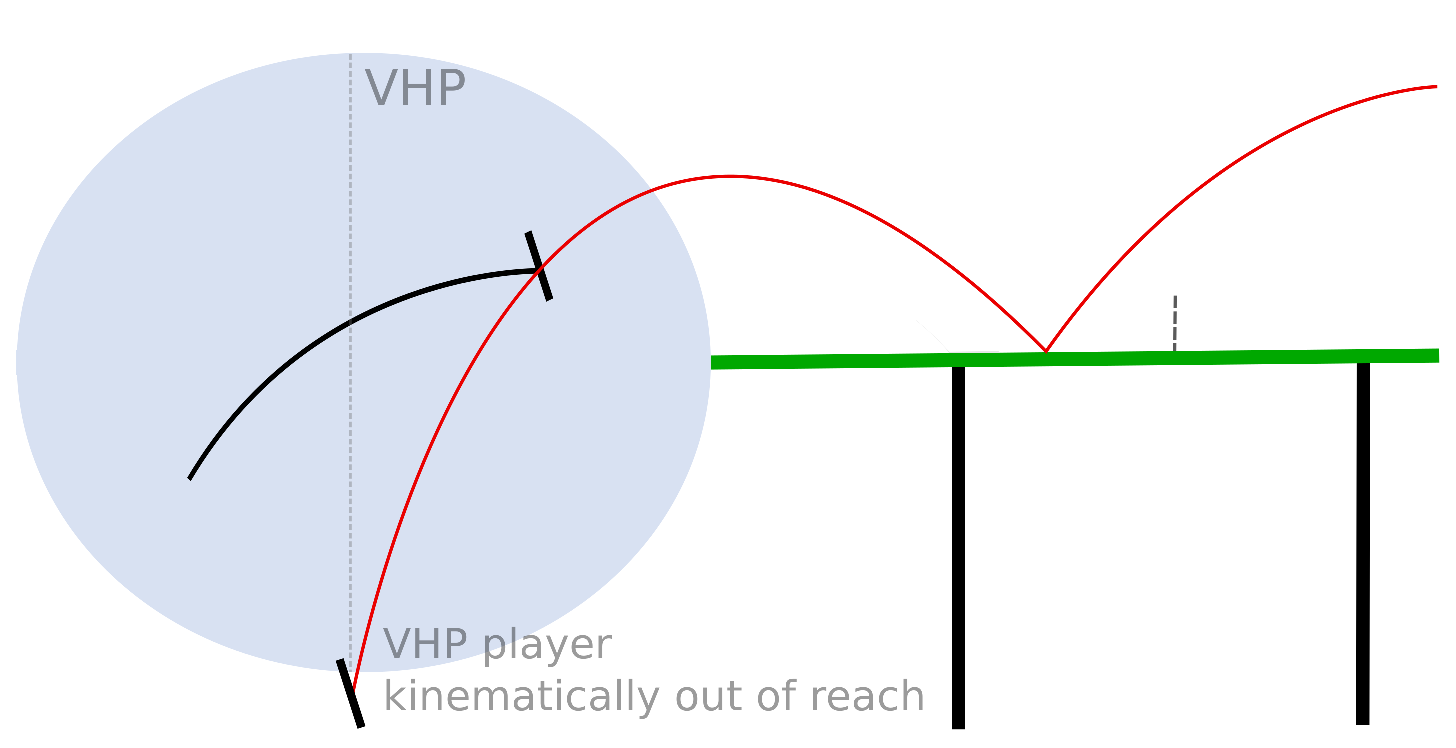
\includegraphics[scale=0.30]{drawingUpdate.eps}			
\caption{Fixing a virtual hitting plane (VHP) can make the generated trajectories unnecessarily restrictive and the resulting inverse kinematics may be infeasible. Instead the whole ball trajectory should be considered in a trajectory generation framework and the hitting time as well as the hitting point should be optimized. The predicted ball trajectory and a feasible racket trajectory are shown in red and black, respectively. VHP is shown as a dotted gray line, the workspace of the robot is shown as an ellipsoidal light blue region.}
\label{mainIdea}
\end{figure}